\newpage
\section{Innledning}
Rapporten vurderer systempåliteligheten til et kompressortog bestående av to kompressorer og én felles drivenhet, installert på en oljeplattform. Kompressorene benyttes til å komprimere gass for reinjisering i et reservoar. Systemet består av en førstetrinns kompressor, en andretrinns kompressor og en elmotor drevet av en gassturbin. For at kompressortoget skal fungere, må begge kompressorene og drivenheten være operative.

Først beregnes påliteligheten til eksisterende seriesystem. Deretter vurderes ulike redundansløsninger, og alternativene sammenlignes med hensyn til økt systempålitelighet, reparasjonstid og praktiske begrensninger.

\section{Teori}

Et seriesystem er et system der hver komponent må fungere for at systemet som helhet skal fungere \parencite{pedersen_syspal}. Kompressortoget i denne oppgaven modelleres som et seriesystem fordi begge kompressorene og drivenheten må være operative for at gass skal kunne komprimeres og reinjiseres.

Systempålitelighet er sannsynligheten for at et system fungerer uten feil over en gitt tidsperiode \parencite{pedersen_syspal}. Hver komponent har en egen pålitelighet, og sammensettingen av komponentene påvirker systemets samlede pålitelighet. For eksempel vil to like komponenter koblet i serie gi en annen pålitelighet enn de samme komponentene koblet i parallell. I beregningene forutsettes det at komponentfeilene er uavhengige av hverandre.

Systempåliteligheten til et seriesystem $R_{\text{sys}}$ beregnes som produktet av komponentenes påliteligheter $R_i$:
\begin{equation}
R_{\text{sys}} = \prod_{i=1}^{n} R_i
\end{equation}
$R_{\text{sys}}$ avtar med økende antall seriekoblede komponenter med pålitelighet $<$ 100\%. Desto lavere pålitelighet en komponent har, desto større effekt vil dette ha på påliteligheten til systemet.

Systempåliteligheten til et parallellkoblet system er uttrykt som:
\begin{equation}
R_{\text{par}} = 1 - \prod_{i=1}^{n} (1 - R_i)
\end{equation}
$R_{\text{par}}$ øker med økende antall parallellkoblede komponenter \parencite{pedersen_syspal}. Økningen av pålitelighet til systemet, i prosentpoeng, er størst for parallellkobling av de minst pålitelige individuelle komponentene.

Redundans innebærer at en ekstra komponent legges til for å sikre systemfunksjonen dersom den primære feiler \parencite{pedersen_redundans}.

Det er viktig å skille mellom pålitelighet og tilgjengelighet. Pålitelighet beskriver sannsynligheten for feilfri drift over en periode, mens tilgjengelighet beskriver hvor stor andel av tiden systemet faktisk er operativt, og avhenger også av reparasjonstid. Mean Time To Repair (MTTR) er forventet reparasjonstid etter feil for en enkelt komponent.

\section{Metode}
\subsection{Nåværende systempålitelighet for kompressortoget}

Kompressortoget består av tre separate komponenter, og modelleres som et seriesystem. Systempåliteligheten $R_{\text{sys}}$ beregnes derfor som produktet av komponentenes påliteligheter, via formel (1). Ved å multiplisere sammen påliteligheten til hver komponent får vi:
\[
R_{\text{sys}} = 0{,}95 \cdot 0{,}90 \cdot 0{,}89 = 0{,}76095 \approx 0{,}761
\]

\begin{table}[H]
    \centering
    \caption{Pålitelighetsdata og systempålitelighet for kompressortoget}
    \label{tab:palitelighet}
    \begin{tabular}{lcc}
        \hline
        \textbf{Enhet} & \textbf{Pålitelighet, $R_i$} & \textbf{MTTR (timer)} \\
        \hline
        Første trinns kompressor & 0{,}95 & 40 \\
        Andre trinns kompressor  & 0{,}90 & 16 \\
        Elmotor                  & 0{,}89 & 4  \\
        \hline
        \textbf{Seriesystem, $R_{\text{sys}}$} & \textbf{0{,}76095} & --- \\
        \hline
    \end{tabular}
\end{table}

Systempåliteligheten til det eksisterende kompressortoget er dermed omtrent $76\%$.


\subsection{Tiltak for forbedret systempålitelighet}

Forbedring av systempåliteligheten kan oppnås ved å parallellkoble en identisk komponent med en eksisterende komponent \parencite{pedersen_redundans}. Når en komponent feiler, kan reservekomponenten ta over arbeidet. Om mer enn én komponent parallellkobles i kompressortoget, er det ønskelig å koble reservekomponenten sammen med de andre leddene, slik at den sekundære komponenten fungerer som en komplett reserve for den primære.

For hvert redundansscenario ble først den parallelle komponentpåliteligheten beregnet ved hjelp av formel (2). Deretter ble denne satt inn i seriesystemet sammen med de øvrige komponentene.

Påliteligheten til kompressortoget kan nå følgende verdier gitt parallellkoblingene som er nevnt i tabellen under.

\begin{table}[H]
    \centering
    \caption{Systempålitelighet ved ulike redundansløsninger}
    \label{tab:redundans}
    \begin{tabular}{lc}
        \hline
        \textbf{Scenario} & \textbf{$R_{\text{sys}}$} \\
        \hline
        \multicolumn{2}{l}{\textit{Én komponent parallellkoblet}} \\
        Første trinns kompressor        & 79{,}89\,\% \\
        Andre trinns kompressor         & 83{,}70\,\% \\
        Elmotor                         & 84{,}47\,\% \\
        \hline
        \multicolumn{2}{l}{\textit{To komponenter parallellkoblet}} \\
        Begge kompressorene             & 87{,}89\,\% \\
        Første trinns kompressor og elmotor  & 88{,}69\,\% \\
        Andre trinns kompressor og elmotor   & 92{,}91\,\% \\
        \hline
        \multicolumn{2}{l}{\textit{Alle tre komponenter parallellkoblet}} \\
        Alle komponenter                & 97{,}56\,\% \\
        \hline
    \end{tabular}
\end{table}

%BILDE HER MAST1102 DV Oppgave 3 Tabell
\begin{figure}[h]
\centering
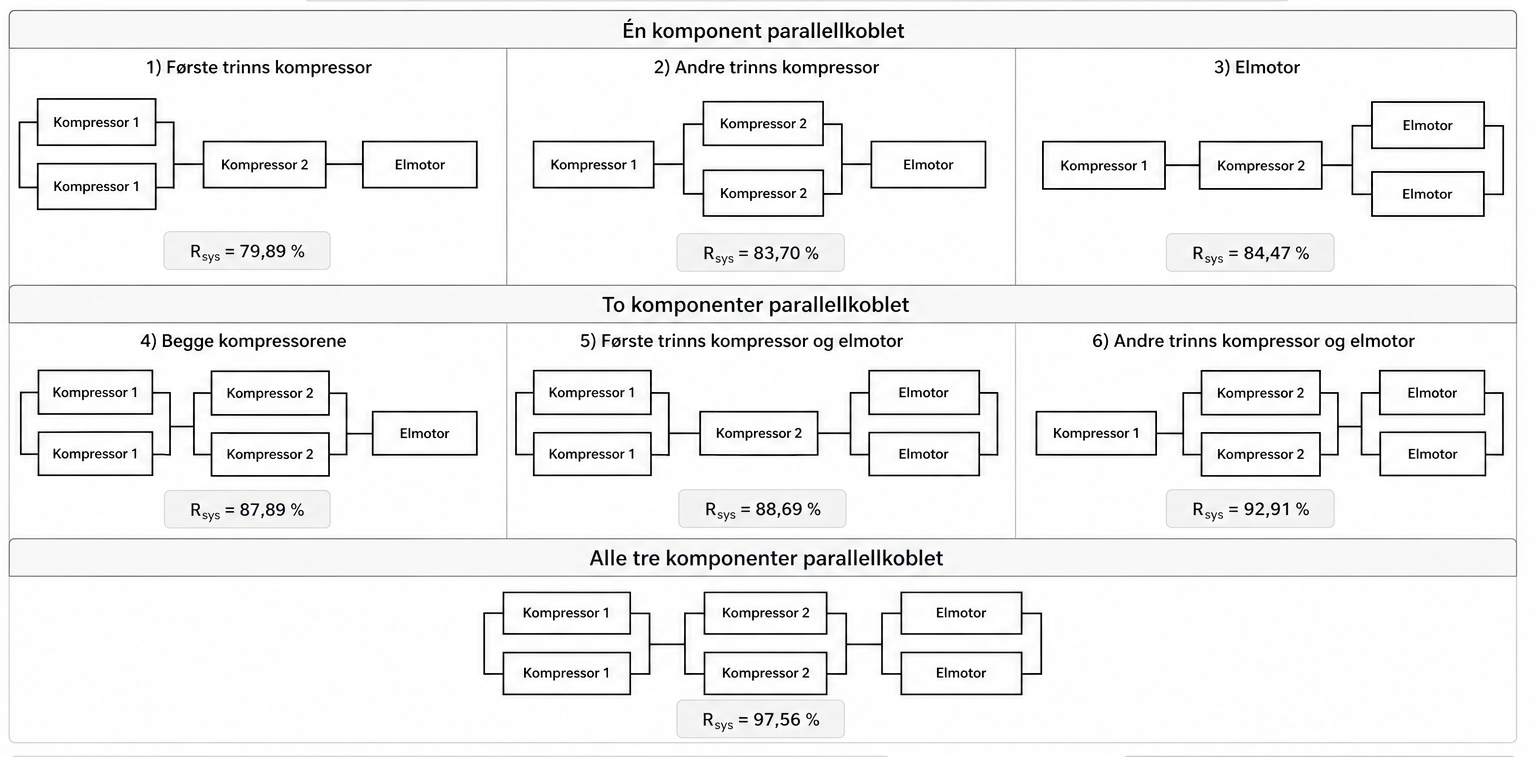
\includegraphics[width=1.0\linewidth]{MAST1102 DV Oppgave 3 Tabell.png}
\caption{Grafisk fremstilling av Tabell 2}
\label{fig:mast1102}
\end{figure}

Avhengig av hvilke komponenter som parallellkobles, kan systempåliteligheten økes fra omtrent 80\% til 98\%.

Beregningene forutsetter at redundante komponenter er uavhengige og identiske med de opprinnelige komponentene. I praksis kan dette være en forenkling. På en oljeplattform kan fellesfeil, begrenset plass, økt vekt, økt vedlikeholdsbehov og høy investeringskostnad redusere nytteverdien av redundans. Beregningene er en ren teknisk sammenligning — vi har ikke sett på kostnader.

\section{Diskusjon}

Resultatene viser at systempåliteligheten forbedres mest ved å parallellkoble de minst pålitelige komponentene. Redundans på andretrinns kompressoren og elmotoren gir en økning i pålitelighet fra 76\% til 93\%. En ytterligere parallellkobling av førstetrinns kompressoren gir en økning til omtrent 98\%.

Førstetrinns kompressor har den lengste reparasjonstiden (MTTR = 40 timer). Dersom begge kompressorene får redundans, vil en feil i én kompressor i større grad kunne håndteres uten umiddelbar stans i kompressortoget. Dette kan redusere konsekvensen av de lange reparasjonstidene for kompressorene. Likevel er det ikke beregnet en samlet systemtilgjengelighet i denne rapporten, og MTTR-verdiene bør derfor tolkes som et beslutningsgrunnlag, ikke som direkte system-MTTR.

Her må det vurderes om ønsket pålitelighet, reparasjonstid og andre begrensninger som plass, vekt, investeringskostnad, økt vedlikeholdsbehov og risiko for fellesfeil veier inn på valg av løsning. Tre forslag presenteres:

\textbf{\large Forslag 1 - Full redundans}

Alle tre komponentene parallellkobles. Som tabell~\ref{tab:redundans} viser gir dette høyest pålitelighet, men det krever dobling av alle komponenter. Det må vurderes om plass, vekt og risiko for fellesfeil på plattformen tillater et slikt inngrep.

\textbf{\large Forslag 2 - Prioritere pålitelighet}

Andretrinns kompressoren og elmotoren parallellkobles. Dette gir nest høyest pålitelighet ved bare fem komponenter, og er billigere og lettere enn full redundans. Førstetrinns kompressor har fortsatt MTTR på 40 timer, så en feil der kan gi lengre nedetid.

\textbf{\large Forslag 3 - Prioritere MTTR}

Begge kompressorene parallellkobles. Påliteligheten er lavere enn i forslag 2, men redundansen gjør at en kompressorfeil ikke nødvendigvis stopper toget. Flaskehalsen for reparasjonstid blir da elmotoren med MTTR på bare 4 timer.

\section{Konklusjon}

Systempåliteligheten til kompressortoget kan økes en god del ved parallellkobling av redundante komponenter. Dersom målet utelukkende er høyest systempålitelighet, er full redundans det beste alternativet, med beregnet pålitelighet på 97{,}56\%. Dersom kostnad, plass og vekt vektlegges, fremstår redundans på andretrinns kompressor og elmotor som et mer balansert tiltak, siden dette øker systempåliteligheten fra 76{,}10\% til 92{,}91\% uten å doble hele kompressortoget. Redundans på begge kompressorene kan være aktuelt dersom hovedmålet er å redusere konsekvensen av lang reparasjonstid, men dette gir lavere beregnet pålitelighet enn alternativet med redundans på andretrinns kompressor og elmotor. Beregningene er basert på idealiserte forutsetninger om uavhengige og identiske komponenter, og en fullstendig vurdering bør også inkludere praktiske begrensninger og økonomiske analyser.
